\documentclass[11pt,english]{article}
%\usepackage{times}
\usepackage[T1]{fontenc}
\usepackage[authoryear]{natbib}
\usepackage{amssymb,amsmath,amsthm}
%\usepackage[nolists]{endfloat}
\usepackage{graphicx}
\usepackage{chngpage}
\usepackage[hang, small]{caption} % Custom captions under/above floats in tables or figures
\usepackage{pdflscape}
\usepackage{longtable}
\usepackage{color}
\usepackage{epigraph}
\usepackage{float}
\usepackage{array}
\usepackage{fullpage}
\usepackage{setspace}
\usepackage[normalem]{ulem}
\usepackage{appendix}
\usepackage{booktabs}
\usepackage{multirow}
\usepackage[small,compact]{titlesec}
\usepackage{rotate}
\usepackage{subcaption}
\usepackage{titletoc}
\usepackage[pdfborder={0 0 0}]{hyperref}


\newtheorem{definition}{Definition}
\newtheorem{hypothesis}{Hypothesis}
\newtheorem{lemma}{Lemma}
\newtheorem{corollary}{Corollary}
\newtheorem{theorem}{Theorem}

\setlength{\epigraphwidth}{.5\textwidth}


\newcommand{\note}[1]{
  {\color{red} #1 }
}

\begin{document}

\title{Modern Man Challenge: Preliminary Results}

\author{
  Jeannie Annan\footnote{International Rescue Committee and University of Chicago, \href{Jeannie.Annan@rescue.org}{Jeannie.Annan@rescue.org}} \quad  
  Gunther Fink\footnote{Swiss Tropical and Public Health Institute, \href{guenther.fink@swisstph.ch }{guenther.fink@swisstph.ch }} \quad  
  Betsy Levy Paluck\footnote{Princeton University, \href{epaluck@princeton.edu}{epaluck@princeton.edu}}\thanks{
  [THANKS]
  } 
}


\maketitle

%\textbf{Keywords}: ***

%\begin{abstract}
%  ABSTRACT
%\end{abstract}


\clearpage

\tableofcontents

\newpage

\listoftables

\newpage

\setcounter{page}{1}

\doublespacing 

\section{Main Analysis}

\subsection{Regression specifications}

Pre-liminary results are estimated using two different regressions specifications. The unadjusted estimator is a least squares regression that conditions on an indicator for the treatment assignment $Z_i$ and uses CR2 cluster robust standard errors, i.e.:

\[\textrm{IPV}_{ij} = \beta_0 + \beta_1 Z_i + \varepsilon_i \]

The adjusted estimator conditions on mean-centered pre-treatment violence outcomes (i.e. prior to Christmas 2018) that were measured retrospectively during the women's survey and includes interaction terms as suggested in Lin (2013):
\[\textrm{IPV}_{ij} = \beta_0 + \beta_1 Z_i + \beta_2 \overline{X}_i + \beta_3 Z_i \overline{X}_i + \varepsilon_i\]

In both specifications $\beta_1$ estimates the intention-to-treat effect of the Modern Man Challenge. An additional pooled analysis is also presented in which outcomes are aggregated at the cluster level and then regressed using both specifications listed above but at the cluster-level instead of the individual.

\subsection{Any Violence}

\subsubsection{IPV}

\begin{table}[H]
\centering

\begin{tabular}{l c c c c c c}
\toprule
 & IPV & IPV & Physical/Sexual & Physical/Sexual & Emotional & Emotional \\
\midrule
MMC                 & $0.142$        & $0.133$       & $0.111$        & $0.106$       & $0.110$        & $0.066$       \\
                    & $(0.085)$      & $(0.156)$     & $(0.141)$      & $(0.133)$     & $(0.059)$      & $(0.125)$     \\
Constant            & $-0.083$       & $-0.078$      & $-0.086$       & $-0.066$      & $-0.037$       & $-0.034$      \\
                    & $(0.064)$      & $(0.074)$     & $(0.063)$      & $(0.081)$     & $(0.054)$      & $(0.067)$     \\
\midrule
Bootstrap $p$-value & $0.123$        & $0.422$       & $0.406$        & $0.456$       & $0.086$        & $0.631$       \\
Covariates          & $\textrm{Yes}$ & $\textrm{No}$ & $\textrm{Yes}$ & $\textrm{No}$ & $\textrm{Yes}$ & $\textrm{No}$ \\
Clusters            & $16$           & $16$          & $16$           & $16$          & $16$           & $16$          \\
Observations        & $455$          & $455$         & $455$          & $455$         & $455$          & $455$         \\
Adj. R$^2$          & $0.422$        & $0.003$       & $0.386$        & $0.002$       & $0.416$        & $-0.001$      \\
\bottomrule
\multicolumn{7}{l}{\scriptsize{\parbox{\linewidth}{\vspace{2pt} 
       \textit{Notes:} Estimates of the intent-to-treat effects of Modern Man mobile 
       messaging program on pre-registered primary outcomes using adjusted regression 
       specification based on the Lin 2013 estimator with CR2 cluster-robust 
       standard errors in parentheses. Columns 1 and 2 are a composite index of 
       acts of intimate partner violence. Columns 3 and 4 are a composite index of acts
       of physical violence. Columns 5 and 6 are a composite index of acts of sexual violence.
       All indices were constructed using the first factor from IRT models of subitems. 
       Bootstrap $p$-value estimated using 10,000 replicates of wild cluster bootstrap-$t$. \\ $^{***}p<0.001$; $^{**}p<0.01$; $^{*}p<0.05$.}}}
\end{tabular}

\caption{Effects on proportion of women experiencing any IPV since Christmas 2018.}
\label{tab:ipv}
\end{table}

\begin{figure}[H]
\centering
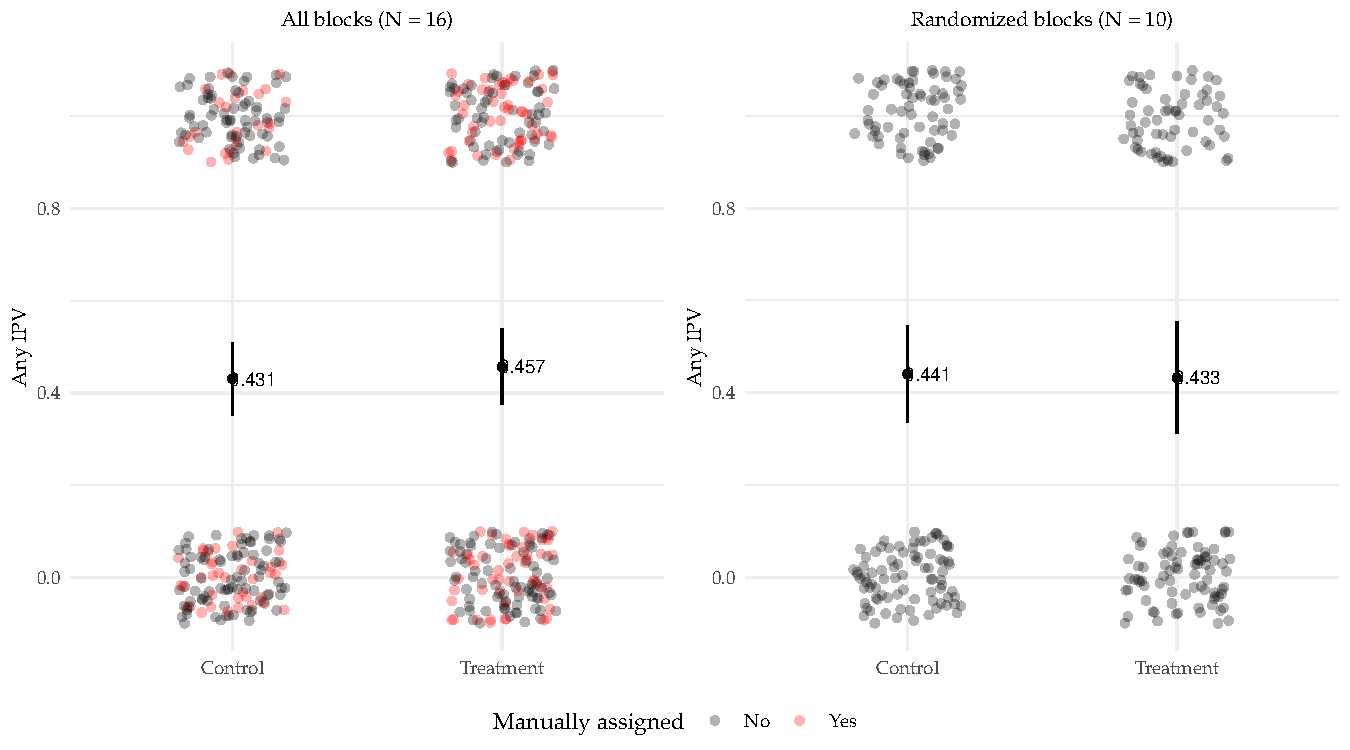
\includegraphics[width = \textwidth]{figures/ipv_plot.pdf}
\caption{Plot of raw data for any IPV outcome.}
\label{fig:ipv_plot}
\end{figure}

\subsubsection{Physical Violence}

\begin{table}[H]
\centering

\begin{tabular}{l c c c c}
\toprule
 & (1) & (2) & (3) & (4) \\
\midrule
MMC          & $0.039$       & $0.049$        & $-0.001$      & $0.015$        \\
             & $(0.057)$     & $(0.052)$      & $(0.085)$     & $(0.074)$      \\
Constant     & $0.312^{***}$ & $0.307^{***}$  & $0.346^{**}$  & $0.334^{**}$   \\
             & $(0.044)$     & $(0.032)$      & $(0.054)$     & $(0.035)$      \\
\midrule
Covariates   & $\textrm{No}$ & $\textrm{Yes}$ & $\textrm{No}$ & $\textrm{Yes}$ \\
Clusters     & $16$          & $16$           & $10$          & $10$           \\
Observations & $463$         & $463$          & $295$         & $295$          \\
Adj. R$^2$   & $-0.000$      & $0.326$        & $-0.003$      & $0.326$        \\
\bottomrule
\multicolumn{5}{l}{\scriptsize{\parbox{.5\linewidth}{\vspace{2pt} 
       \textit{Notes:} Columns 1 and 2 estimate the effect on the full sample while Columns 3 
       and 4 estimate effects among the subset of clusters that were randomly allocated.
       Columns 1 and 3 use the unadjusted estimator while Columns 2 and 4 condition on 
       pre-treatment violence outcomes using the adjusted estimator. Cluster-robust 
       standard errors for all estimates are reported in parentheses. \\ $^{***}p<0.001$; $^{**}p<0.01$; $^{*}p<0.05$.}}}
\end{tabular}

\caption{Effects on proportion of women experiencing any physical violence since Christmas 2018.}
\label{tab:physical}
\end{table}

\subsubsection{Sexual Violence}

\begin{table}[H]
\centering

\begin{tabular}{l c c c c}
\toprule
 & (1) & (2) & (3) & (4) \\
\midrule
MMC          & $0.006$       & $0.014$        & $0.005$       & $0.001$        \\
             & $(0.065)$     & $(0.026)$      & $(0.088)$     & $(0.033)$      \\
Constant     & $0.236^{***}$ & $0.233^{***}$  & $0.243^{**}$  & $0.245^{***}$  \\
             & $(0.028)$     & $(0.020)$      & $(0.033)$     & $(0.021)$      \\
\midrule
Covariates   & $\textrm{No}$ & $\textrm{Yes}$ & $\textrm{No}$ & $\textrm{Yes}$ \\
Clusters     & $16$          & $16$           & $10$          & $10$           \\
Observations & $460$         & $460$          & $293$         & $293$          \\
Adj. R$^2$   & $-0.002$      & $0.582$        & $-0.003$      & $0.597$        \\
\bottomrule
\multicolumn{5}{l}{\scriptsize{\parbox{.5\linewidth}{\vspace{2pt} 
       \textit{Notes:} Columns 1 and 2 estimate the effect on the full sample while Columns 3 
       and 4 estimate effects among the subset of clusters that were randomly allocated.
       Columns 1 and 3 use the unadjusted estimator while Columns 2 and 4 condition on 
       pre-treatment violence outcomes using the adjusted estimator. Cluster-robust 
       standard errors for all estimates are reported in parentheses. \\ $^{***}p<0.001$; $^{**}p<0.01$; $^{*}p<0.05$.}}}
\end{tabular}

\caption{Effects on proportion of women experiencing any sexual violence since Christmas 2018.}
\label{tab:sexual}
\end{table}

%Comments on Table \ref{tab:ipv}
%\begin{itemize}
%  \singlespacing
%  \item All effects are in hypothesized direction. 
%  \item The 
%  \item We s
%\end{itemize}

\subsubsection{Individual Acts}

\begin{figure}[H]
\centering
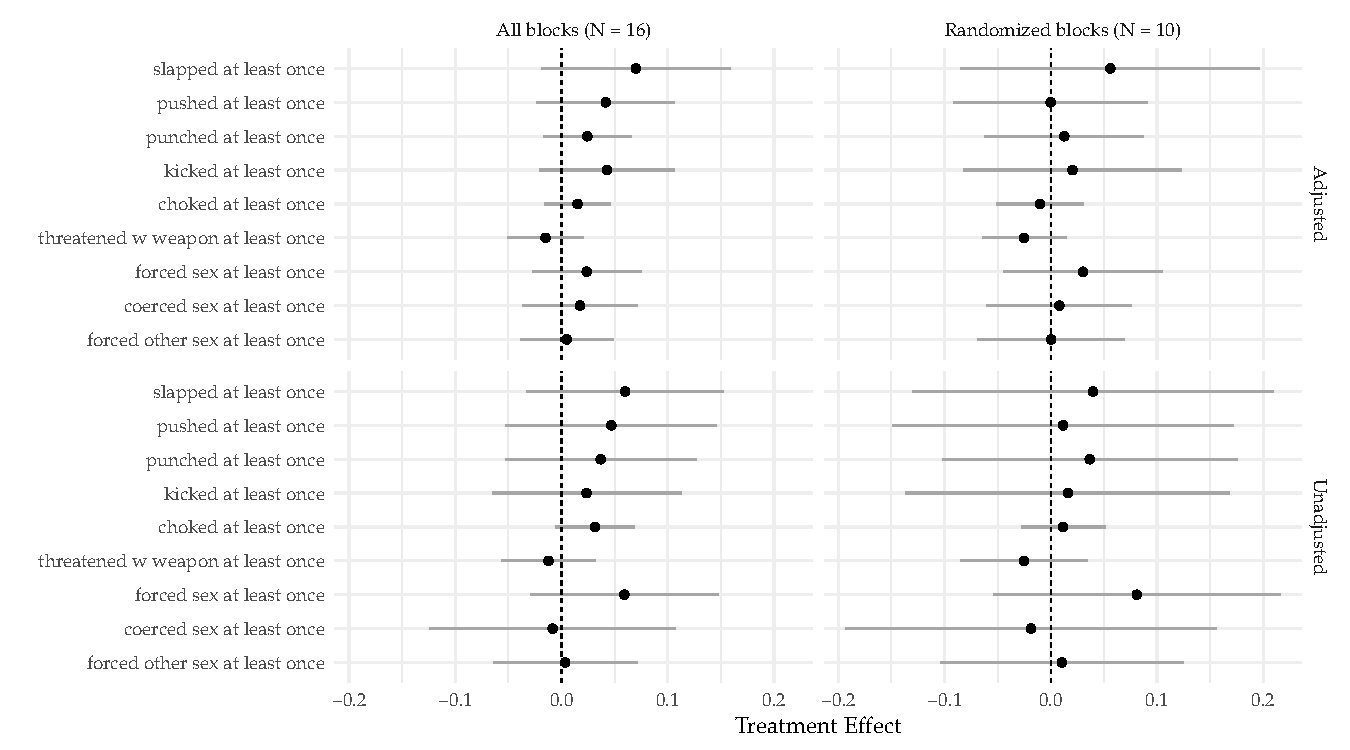
\includegraphics[width = \textwidth]{figures/subitem_plot.pdf}
\caption{Treatment effects on "Any IPV" index items.}
\label{fig:subitems_plot}
\end{figure}

\subsection{Frequency and Breadth of Violence}

\subsubsection{IPV}

\begin{table}[H]
\centering

\begin{tabular}{l c c c c}
\toprule
 & (1) & (2) & (3) & (4) \\
\midrule
MMC          & $0.515$       & $0.437$        & $0.387$       & $0.092$        \\
             & $(0.625)$     & $(0.368)$      & $(0.905)$     & $(0.553)$      \\
Constant     & $1.810^{**}$  & $1.861^{**}$   & $1.961^{*}$   & $2.114^{*}$    \\
             & $(0.320)$     & $(0.323)$      & $(0.428)$     & $(0.437)$      \\
\midrule
Covariates   & $\textrm{No}$ & $\textrm{Yes}$ & $\textrm{No}$ & $\textrm{Yes}$ \\
Clusters     & $16$          & $16$           & $10$          & $10$           \\
Observations & $459$         & $459$          & $293$         & $293$          \\
Adj. R$^2$   & $0.003$       & $0.414$        & $-0.001$      & $0.397$        \\
\bottomrule
\multicolumn{5}{l}{\scriptsize{\parbox{.5\linewidth}{\vspace{2pt} 
       \textit{Notes:} Columns 1 and 2 estimate the effect on the full sample while Columns 3 
       and 4 estimate effects among the subset of clusters that were randomly allocated.
       Columns 1 and 3 use the unadjusted estimator while Columns 2 and 4 condition on 
       pre-treatment violence outcomes using the adjusted estimator. Cluster-robust 
       standard errors for all estimates are reported in parentheses. \\ $^{***}p<0.001$; $^{**}p<0.01$; $^{*}p<0.05$.}}}
\end{tabular}

\caption{Effects on frequency and breadth of IPV since Christmas 2018.}
\label{tab:ipv}
\end{table}

\begin{figure}[H]
\centering
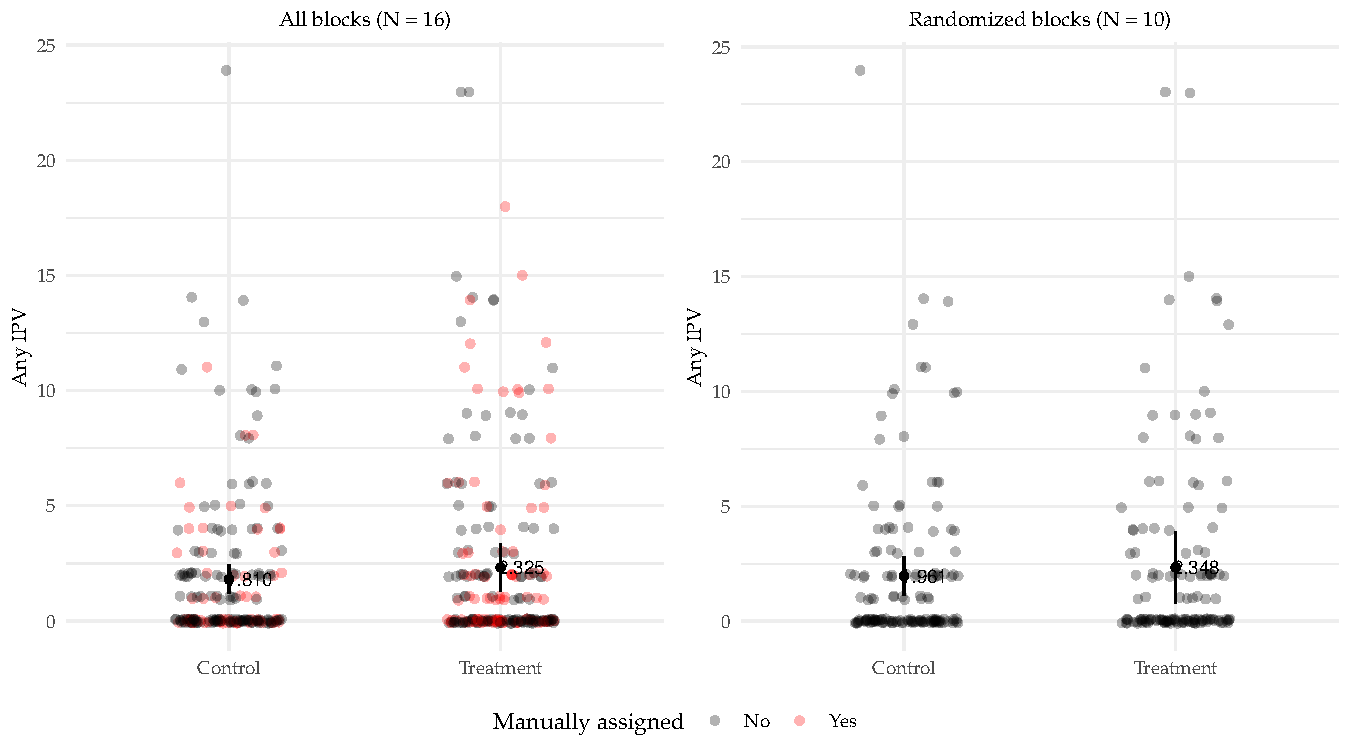
\includegraphics[width = \textwidth]{figures/ipv_freq_plot.pdf}
\caption{Plot of raw data for breadth and frequency of IPV outcome.}
\label{fig:ipv_freq_plot}
\end{figure}

\subsubsection{Physical Violence}

\begin{table}[H]
\centering

\begin{tabular}{l c c c c}
\toprule
 & (1) & (2) & (3) & (4) \\
\midrule
MMC          & $0.436$       & $0.380$        & $0.194$       & $0.050$        \\
             & $(0.340)$     & $(0.255)$      & $(0.529)$     & $(0.358)$      \\
Constant     & $1.193^{***}$ & $1.216^{***}$  & $1.320^{**}$  & $1.415^{**}$   \\
             & $(0.194)$     & $(0.200)$      & $(0.247)$     & $(0.238)$      \\
\midrule
Covariates   & $\textrm{No}$ & $\textrm{Yes}$ & $\textrm{No}$ & $\textrm{Yes}$ \\
Clusters     & $16$          & $16$           & $10$          & $10$           \\
Observations & $463$         & $463$          & $295$         & $295$          \\
Adj. R$^2$   & $0.003$       & $0.368$        & $-0.002$      & $0.333$        \\
\bottomrule
\multicolumn{5}{l}{\scriptsize{\parbox{.5\linewidth}{\vspace{2pt} 
       \textit{Notes:} Columns 1 and 2 estimate the effect on the full sample while Columns 3 
       and 4 estimate effects among the subset of clusters that were randomly allocated.
       Columns 1 and 3 use the unadjusted estimator while Columns 2 and 4 condition on 
       pre-treatment violence outcomes using the adjusted estimator. Cluster-robust 
       standard errors for all estimates are reported in parentheses. \\ $^{***}p<0.001$; $^{**}p<0.01$; $^{*}p<0.05$.}}}
\end{tabular}

\caption{Effects on frequency and breadth of physical violence since Christmas 2018.}
\label{tab:physical}
\end{table}

\subsubsection{Sexual Violence}

\begin{table}[H]
\centering

\begin{tabular}{l c c c c}
\toprule
 & (1) & (2) & (3) & (4) \\
\midrule
MMC          & $0.144$       & $0.076$        & $0.191$       & $0.037$        \\
             & $(0.278)$     & $(0.156)$      & $(0.400)$     & $(0.220)$      \\
Constant     & $0.606^{**}$  & $0.645^{**}$   & $0.632^{*}$   & $0.695^{*}$    \\
             & $(0.152)$     & $(0.145)$      & $(0.193)$     & $(0.201)$      \\
\midrule
Covariates   & $\textrm{No}$ & $\textrm{Yes}$ & $\textrm{No}$ & $\textrm{Yes}$ \\
Clusters     & $16$          & $16$           & $10$          & $10$           \\
Observations & $460$         & $460$          & $293$         & $293$          \\
Adj. R$^2$   & $0.000$       & $0.492$        & $0.000$       & $0.460$        \\
\bottomrule
\multicolumn{5}{l}{\scriptsize{\parbox{.5\linewidth}{\vspace{2pt} 
       \textit{Notes:} Columns 1 and 2 estimate the effect on the full sample while Columns 3 
       and 4 estimate effects among the subset of clusters that were randomly allocated.
       Columns 1 and 3 use the unadjusted estimator while Columns 2 and 4 condition on 
       pre-treatment violence outcomes using the adjusted estimator. Cluster-robust 
       standard errors for all estimates are reported in parentheses. \\ $^{***}p<0.001$; $^{**}p<0.01$; $^{*}p<0.05$.}}}
\end{tabular}

\caption{Effects on frequency and breadth of sexual violence since Christmas 2018.}
\label{tab:sexual}
\end{table}

\subsubsection{Individual Acts}

\begin{figure}[H]
\centering
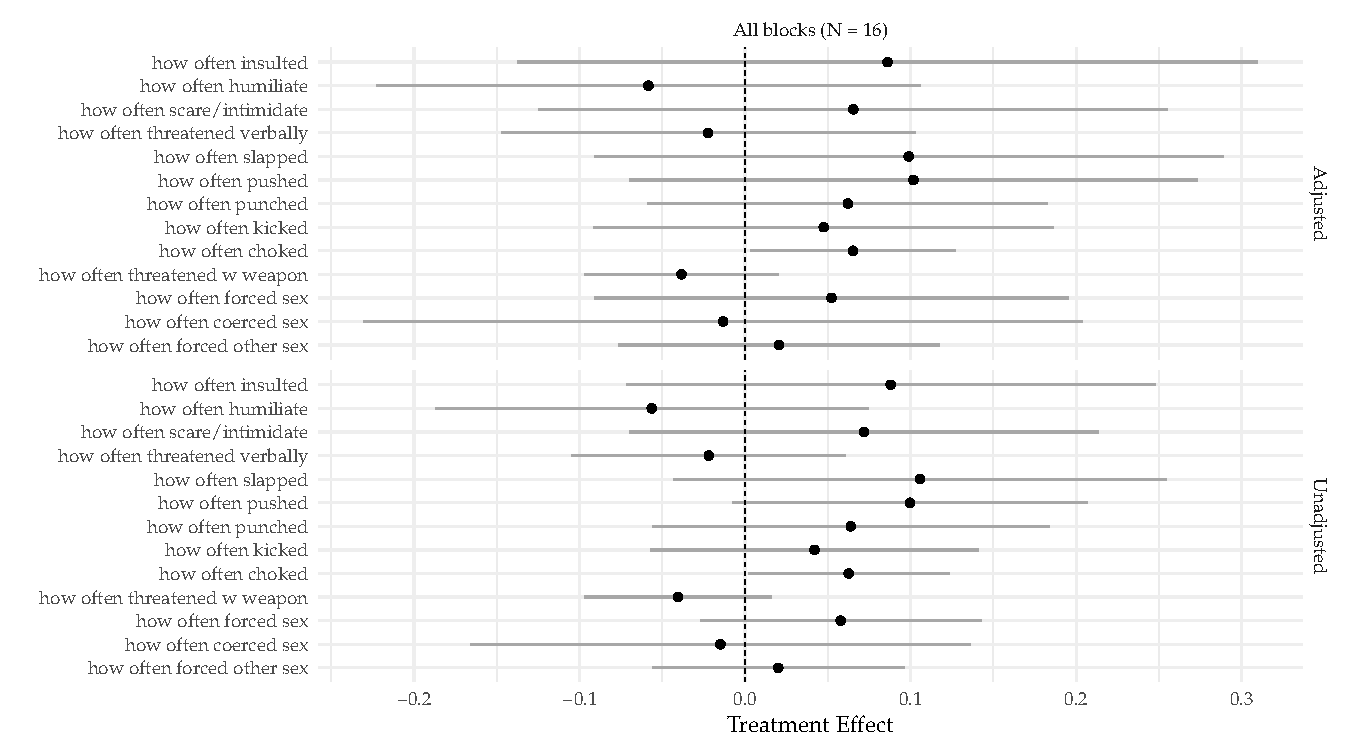
\includegraphics[width = \textwidth]{figures/subitem_freq_plot.pdf}
\caption{Treatment effects on "Frequency and Breadth of IPV" index items.}
\label{fig:subitems_freq_plot}
\end{figure}

\section{Pooled Analysis}

\subsection{Any Violence}

\subsubsection{IPV}

\begin{table}[H]
\centering

\begin{tabular}{l c c c c c c}
\toprule
 & IPV & IPV & Physical/Sexual & Physical/Sexual & Emotional & Emotional \\
\midrule
MMC                 & $0.173$        & $0.151$       & $0.122$        & $0.122$       & $0.093$        & $0.057$       \\
                    & $(0.080)$      & $(0.121)$     & $(0.101)$      & $(0.101)$     & $(0.074)$      & $(0.092)$     \\
Constant            & $-0.083$       & $-0.095$      & $-0.092$       & $-0.092$      & $-0.055$       & $-0.043$      \\
                    & $(0.050)$      & $(0.057)$     & $(0.060)$      & $(0.060)$     & $(0.059)$      & $(0.059)$     \\
\midrule
Bootstrap $p$-value & $0.083$        & $0.230$       & $0.243$        & $0.249$       & $0.293$        & $0.548$       \\
Covariates          & $\textrm{Yes}$ & $\textrm{No}$ & $\textrm{Yes}$ & $\textrm{No}$ & $\textrm{Yes}$ & $\textrm{No}$ \\
Clusters            & $16$           & $16$          & $16$           & $16$          & $16$           & $16$          \\
Observations        & $16$           & $16$          & $16$           & $16$          & $16$           & $16$          \\
Adj. R$^2$          & $0.537$        & $0.036$       & $0.029$        & $0.029$       & $0.527$        & $-0.043$      \\
\bottomrule
\multicolumn{7}{l}{\scriptsize{\parbox{\linewidth}{\vspace{2pt} 
       \textit{Notes:} Estimates of the intent-to-treat effects of Modern Man mobile 
       messaging program on pre-registered primary outcomes with data pooled at the block 
       level and using adjusted regression specification based on the Lin 2013 estimator with 
       CR2 cluster-robust standard errors in parentheses. Columns 1 and 2 are a composite 
       index of acts of intimate partner violence. Columns 3 and 4 are a composite index of acts
       of physical violence. Columns 5 and 6 are a composite index of acts of sexual violence.
       All indices were constructed using the first factor from IRT models of subitems. 
       Bootstrap $p$-value estimated using 10,000 replicates of wild cluster bootstrap-$t$. \\ $^{***}p<0.001$; $^{**}p<0.01$; $^{*}p<0.05$.}}}
\end{tabular}

\caption{Pooled effects on proportion of women experiencing any IPV since Christmas 2018.}
\label{tab:ipv}
\end{table}

\begin{figure}[H]
\centering
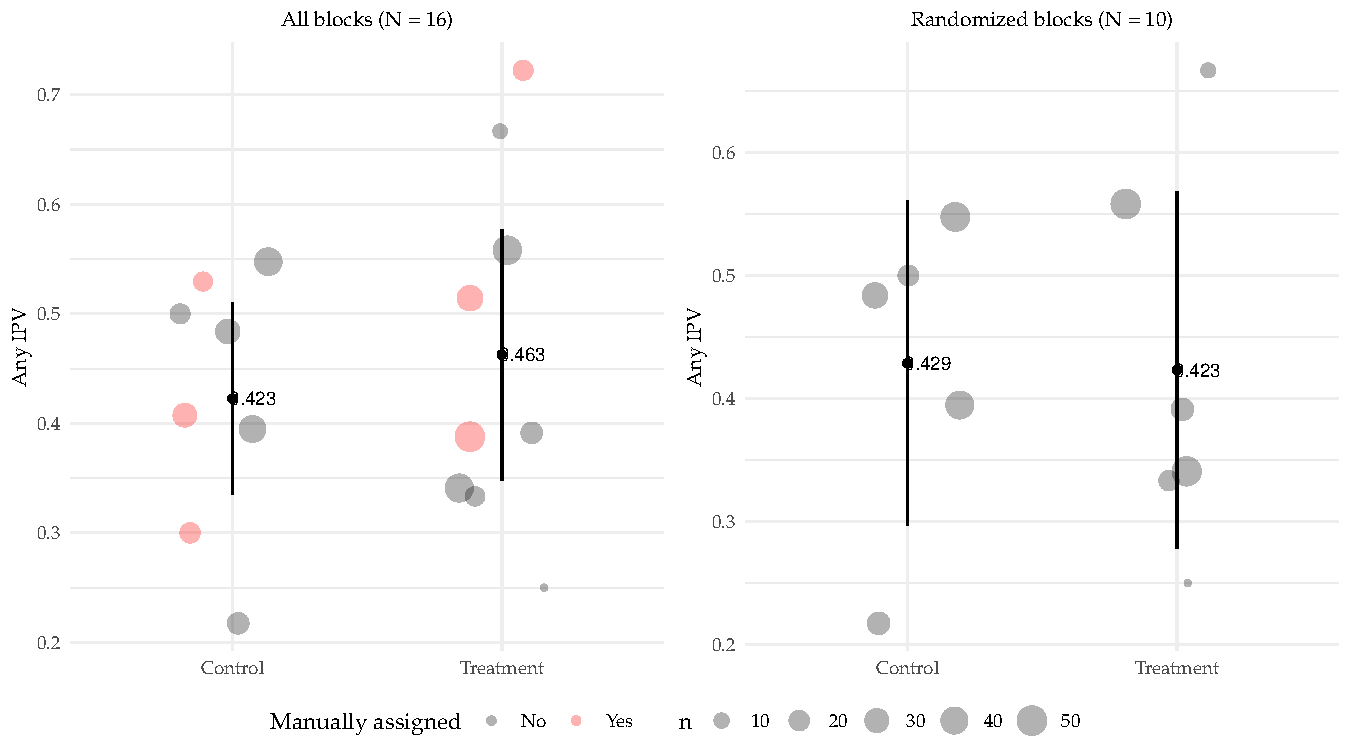
\includegraphics[width = \textwidth]{figures/pooled_ipv_plot.pdf}
\caption{Plot of raw data for any IPV outcome.}
\label{fig:pooled_ipv_plot}
\end{figure}

\subsubsection{Physical Violence}

\begin{table}[H]
\centering

\begin{tabular}{l c c c c}
\toprule
 & (1) & (2) & (3) & (4) \\
\midrule
MMC          & $0.040$       & $0.037$        & $-0.027$      & $-0.021$       \\
             & $(0.053)$     & $(0.046)$      & $(0.068)$     & $(0.052)$      \\
Constant     & $0.293^{***}$ & $0.294^{***}$  & $0.335^{***}$ & $0.331^{***}$  \\
             & $(0.039)$     & $(0.031)$      & $(0.051)$     & $(0.025)$      \\
\midrule
Covariates   & $\textrm{No}$ & $\textrm{Yes}$ & $\textrm{No}$ & $\textrm{Yes}$ \\
Clusters     & $16$          & $16$           & $10$          & $10$           \\
Observations & $17$          & $17$           & $11$          & $11$           \\
Adj. R$^2$   & $-0.027$      & $0.060$        & $-0.092$      & $0.104$        \\
\bottomrule
\multicolumn{5}{l}{\scriptsize{\parbox{.5\linewidth}{\vspace{2pt} 
       \textit{Notes:} Columns 1 and 2 estimate the effect on the full sample while Columns 3 
       and 4 estimate effects among the subset of clusters that were randomly allocated.
       Columns 1 and 3 use the unadjusted estimator while Columns 2 and 4 condition on 
       pre-treatment violence outcomes using the adjusted estimator. Cluster-robust 
       standard errors for all estimates are reported in parentheses. \\ $^{***}p<0.001$; $^{**}p<0.01$; $^{*}p<0.05$.}}}
\end{tabular}

\caption{Pooled effects on proportion of women experiencing any physical violence since Christmas 2018.}
\label{tab:physical}
\end{table}

\subsubsection{Sexual Violence}

\begin{table}[H]
\centering

\begin{tabular}{l c c c c}
\toprule
 & (1) & (2) & (3) & (4) \\
\midrule
MMC          & $0.006$       & $0.021$        & $-0.016$      & $-0.002$       \\
             & $(0.057)$     & $(0.029)$      & $(0.067)$     & $(0.040)$      \\
Constant     & $0.233^{***}$ & $0.230^{***}$  & $0.233^{***}$ & $0.247^{***}$  \\
             & $(0.026)$     & $(0.021)$      & $(0.027)$     & $(0.023)$      \\
\midrule
Covariates   & $\textrm{No}$ & $\textrm{Yes}$ & $\textrm{No}$ & $\textrm{Yes}$ \\
Clusters     & $16$          & $16$           & $10$          & $10$           \\
Observations & $17$          & $17$           & $11$          & $11$           \\
Adj. R$^2$   & $-0.066$      & $0.718$        & $-0.105$      & $0.680$        \\
\bottomrule
\multicolumn{5}{l}{\scriptsize{\parbox{.5\linewidth}{\vspace{2pt} 
       \textit{Notes:} Columns 1 and 2 estimate the effect on the full sample while Columns 3 
       and 4 estimate effects among the subset of clusters that were randomly allocated.
       Columns 1 and 3 use the unadjusted estimator while Columns 2 and 4 condition on 
       pre-treatment violence outcomes using the adjusted estimator. Cluster-robust 
       standard errors for all estimates are reported in parentheses. \\ $^{***}p<0.001$; $^{**}p<0.01$; $^{*}p<0.05$.}}}
\end{tabular}

\caption{Pooled effects on proportion of women experiencing any sexual violence since Christmas 2018.}
\label{tab:sexual}
\end{table}

\subsection{Frequency and Breadth of Violence}

\subsubsection{IPV}

\begin{table}[H]
\centering

\begin{tabular}{l c c c c}
\toprule
 & (1) & (2) & (3) & (4) \\
\midrule
MMC          & $0.448$       & $0.321$        & $0.089$       & $-0.282$       \\
             & $(0.477)$     & $(0.335)$      & $(0.621)$     & $(0.616)$      \\
Constant     & $1.695^{***}$ & $1.706^{***}$  & $1.800^{***}$ & $2.143^{**}$   \\
             & $(0.243)$     & $(0.236)$      & $(0.376)$     & $(0.477)$      \\
\midrule
Covariates   & $\textrm{No}$ & $\textrm{Yes}$ & $\textrm{No}$ & $\textrm{Yes}$ \\
Clusters     & $16$          & $16$           & $10$          & $10$           \\
Observations & $17$          & $17$           & $11$          & $11$           \\
Adj. R$^2$   & $-0.011$      & $0.498$        & $-0.109$      & $0.308$        \\
\bottomrule
\multicolumn{5}{l}{\scriptsize{\parbox{.5\linewidth}{\vspace{2pt} 
       \textit{Notes:} Columns 1 and 2 estimate the effect on the full sample while Columns 3 
       and 4 estimate effects among the subset of clusters that were randomly allocated.
       Columns 1 and 3 use the unadjusted estimator while Columns 2 and 4 condition on 
       pre-treatment violence outcomes using the adjusted estimator. Cluster-robust 
       standard errors for all estimates are reported in parentheses. \\ $^{***}p<0.001$; $^{**}p<0.01$; $^{*}p<0.05$.}}}
\end{tabular}

\caption{Pooled effects on frequency and breadth of IPV since Christmas 2018.}
\label{tab:ipv}
\end{table}

\begin{figure}[H]
\centering
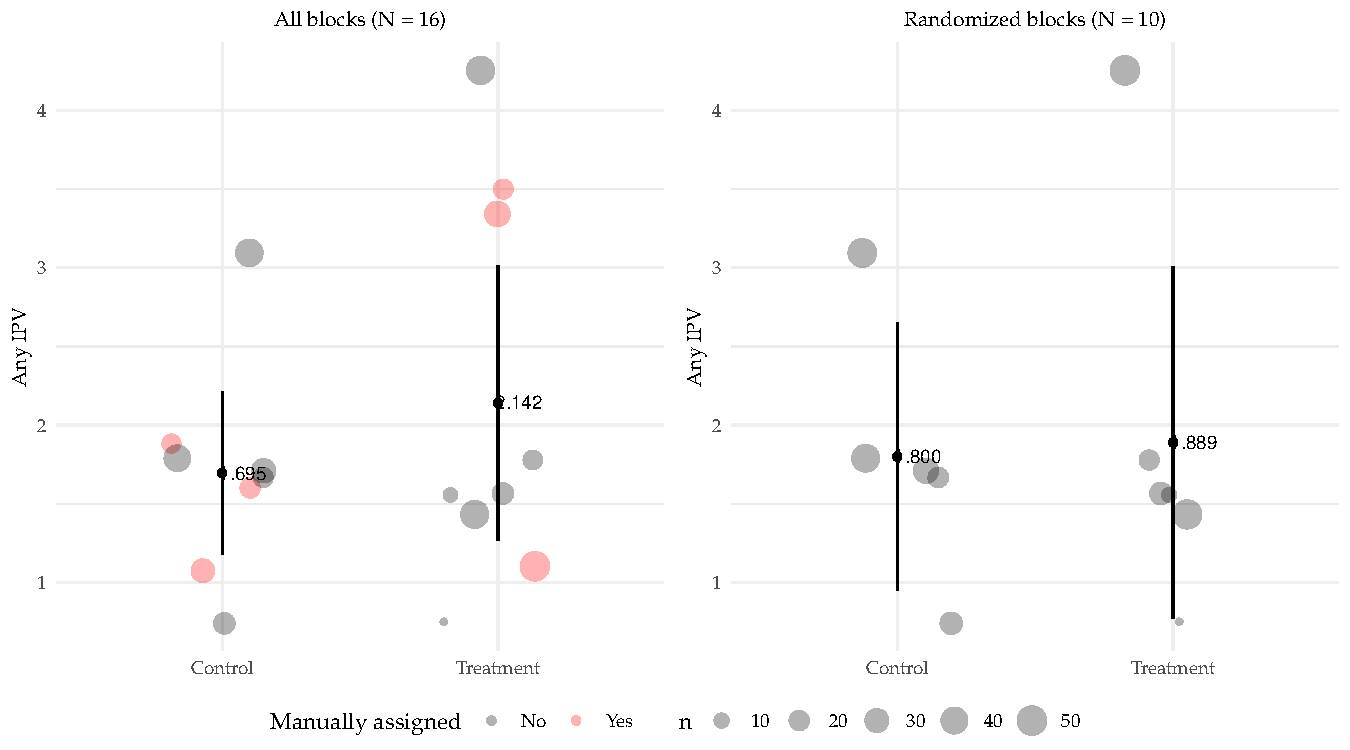
\includegraphics[width = \textwidth]{figures/pooled_ipv_freq_plot.pdf}
\caption{Plot of raw data for breadth and frequency of IPV outcome.}
\label{fig:pooled_ipv_freq_plot}
\end{figure}

\subsubsection{Physical Violence}

\begin{table}[H]
\centering

\begin{tabular}{l c c c c}
\toprule
 & (1) & (2) & (3) & (4) \\
\midrule
MMC          & $0.340$       & $0.259$        & $-0.050$      & $-0.271$       \\
             & $(0.308)$     & $(0.261)$      & $(0.390)$     & $(0.370)$      \\
Constant     & $1.088^{***}$ & $1.092^{***}$  & $1.210^{***}$ & $1.404^{***}$  \\
             & $(0.158)$     & $(0.163)$      & $(0.232)$     & $(0.232)$      \\
\midrule
Covariates   & $\textrm{No}$ & $\textrm{Yes}$ & $\textrm{No}$ & $\textrm{Yes}$ \\
Clusters     & $16$          & $16$           & $10$          & $10$           \\
Observations & $17$          & $17$           & $11$          & $11$           \\
Adj. R$^2$   & $0.009$       & $0.255$        & $-0.109$      & $0.129$        \\
\bottomrule
\multicolumn{5}{l}{\scriptsize{\parbox{.5\linewidth}{\vspace{2pt} 
       \textit{Notes:} Columns 1 and 2 estimate the effect on the full sample while Columns 3 
       and 4 estimate effects among the subset of clusters that were randomly allocated.
       Columns 1 and 3 use the unadjusted estimator while Columns 2 and 4 condition on 
       pre-treatment violence outcomes using the adjusted estimator. Cluster-robust 
       standard errors for all estimates are reported in parentheses. \\ $^{***}p<0.001$; $^{**}p<0.01$; $^{*}p<0.05$.}}}
\end{tabular}

\caption{Pooled effects on frequency and breadth of physical violence since Christmas 2018.}
\label{tab:physical}
\end{table}

\subsubsection{Sexual Violence}

\begin{table}[H]
\centering

\begin{tabular}{l c c c c}
\toprule
 & (1) & (2) & (3) & (4) \\
\midrule
MMC          & $0.139$       & $0.109$        & $0.136$       & $-0.101$       \\
             & $(0.219)$     & $(0.152)$      & $(0.275)$     & $(0.390)$      \\
Constant     & $0.598^{***}$ & $0.609^{***}$  & $0.583^{**}$  & $0.831$        \\
             & $(0.139)$     & $(0.136)$      & $(0.156)$     & $(0.375)$      \\
\midrule
Covariates   & $\textrm{No}$ & $\textrm{Yes}$ & $\textrm{No}$ & $\textrm{Yes}$ \\
Clusters     & $16$          & $16$           & $10$          & $10$           \\
Observations & $17$          & $17$           & $11$          & $11$           \\
Adj. R$^2$   & $-0.040$      & $0.584$        & $-0.084$      & $0.570$        \\
\bottomrule
\multicolumn{5}{l}{\scriptsize{\parbox{.5\linewidth}{\vspace{2pt} 
       \textit{Notes:} Columns 1 and 2 estimate the effect on the full sample while Columns 3 
       and 4 estimate effects among the subset of clusters that were randomly allocated.
       Columns 1 and 3 use the unadjusted estimator while Columns 2 and 4 condition on 
       pre-treatment violence outcomes using the adjusted estimator. Cluster-robust 
       standard errors for all estimates are reported in parentheses. \\ $^{***}p<0.001$; $^{**}p<0.01$; $^{*}p<0.05$.}}}
\end{tabular}

\caption{Pooled effects on frequency and breadth of sexual violence since Christmas 2018.}
\label{tab:sexual}
\end{table}

\section{Covariate Balance}

\subsection{Pre-treatment Violence}

\begin{figure}[H]
\centering
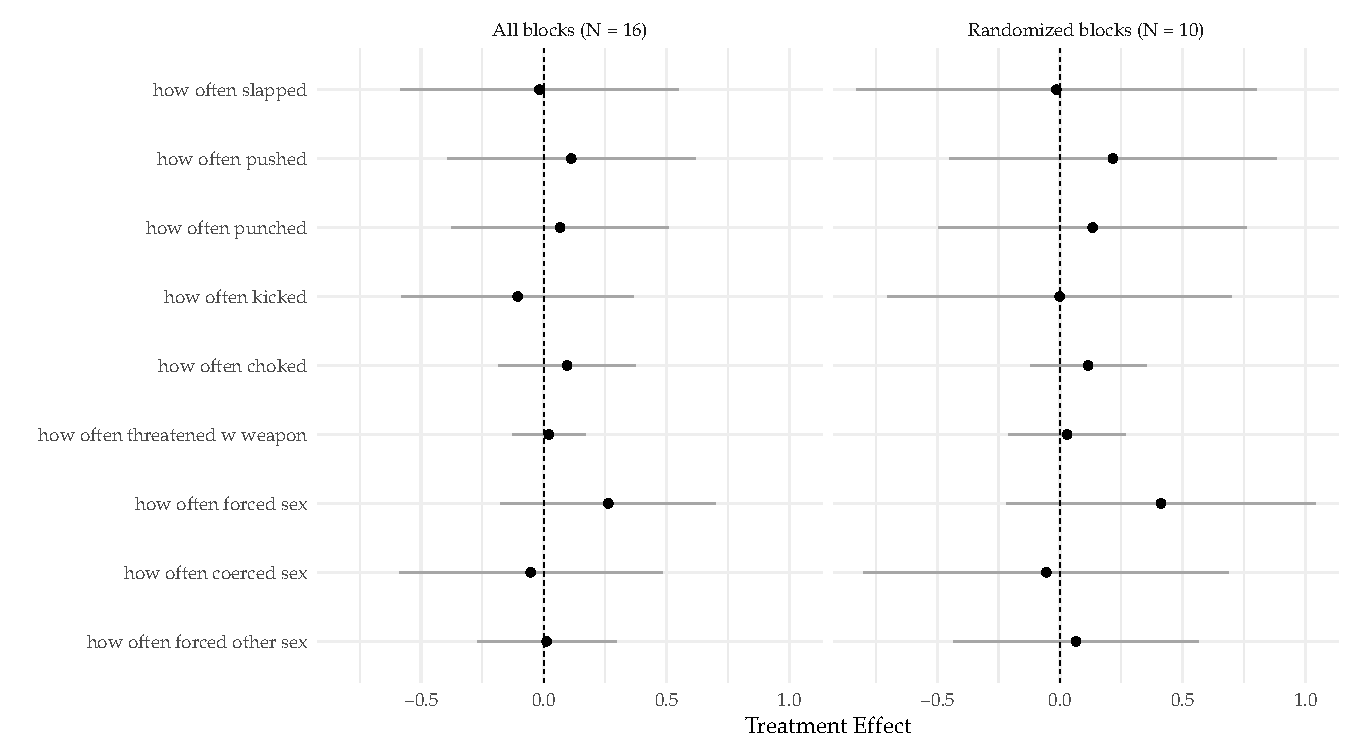
\includegraphics[width = \textwidth]{figures/subitem_balance_plot.pdf}
\caption{Balance on retrospectively reported pre-treatment violence outcomes (i.e. before Christmas 2018).}
\label{fig:subitem_balance_plot}
\end{figure}


\end{document}
